\documentclass[10pt]{book}
\usepackage{graphicx}
\usepackage{exercise}
\usepackage{url}
\usepackage[width=5.5in,height=8.0in,
  hmarginratio=3:2,vmarginratio=1:1]{geometry}


\begin{document}
\chapter {Directed Graphs: A case study of Wikipedia}
\section{Why do directed graphs matter?}
Imagine that it's 2am during finals week, and you're scrambling to finish your research paper on \emph{topica obscura}. Your adrenaline jumps when you finally find a relevant Wikipedia article, with links to more Wikipedia articles! You start clicking away, jumping from page to page in search of facts. An hour later, you realize you're still clicking, but these are pages you've already visited. No matter which link you click, you can't seem to discover any new pages! 

If this situation has ever happened to you, then you've unknowingly (and unfortunately) stumbled upon a knot in Wikipedia. Knots are a unique property of directed graphs. To understand them, it’s necessary to have a basic understanding of directed graphs.
\section{Directed graph implementation}
	 	 	
The graphs we’ve encountered in previous chapters are all undirected graphs. In an undirected graph, a single edge between two vertices represents a symmetric relationship between the vertices. This abstraction works well to describe some real-world systems (such as social networks and transportation networks), but it isn’t detailed enough to describe the Internet, including Wikipedia. Relationships between websites do not have to be symmetric- think of all the pages that Google links to. These pages certainly don't all link back to Google. 

This non-symmetry holds true for Wikipedia as well. Page A might link readers to page B, but page B doesn’t have to include any links to page A. To describe the relationship between pages A and B, we need two bits of information: whether A links to B, and whether B links to A . This is the essence of a directed graph.

\begin{figure}[here]
 \centering
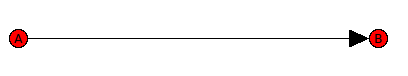
\includegraphics[scale=0.6]{../Images/DirectedGraphExample.png}
\end{figure}
In a directed graph, arcs take on the role of edges. An arc e = (x,y) is an edge from x to y. Arcs are usually referred to as directed edges.

Knots are a unique (and sometimes cruel) property of directed graphs. A knot in a directed graph is a collection of vertices and edges with the property that every vertex in the knot has outgoing edges, and all outgoing edges from vertices in the knot terminate at other vertices in the knot. Thus it is impossible to leave the knot while following the directions of the edges.

We mentioned the idea of knots in Wikipedia. We wondered whether such a thing was even possible? Given that there’s 3,811,000+ articles on Wikipedia, it seemed unlikely that there would be a knot with no outlinks, but we decided to investigate.

Before writing an algorithm to determine the existence of knots in a directed graph, we needed to extend Graph.py to support directed graphs. The result is DirectedGraph.py, which you can download at \url{https://raw.github.com/nrubin/RachelAndNoamsDirectedGraphs/master/DirectedGraph.py}. We recommend reading through DirectedGraph.py and making yourself familiar with the terminology. Note that Edges in DirectedGraph are represented by Arcs.

When we were designing DirectedGraph, we wanted to preserve the order of growth of Vertex and Arc lookups as they were in Graph. Therefore, we decided to keep track of out-arcs in the internal dictionary (inherited from \_\_DictWrapper\_\_), and in-arcs in an extra dictionary, called reverse\_graph. This way, we could keep the lookup of vertices and arcs fast while being able to address out-arcs and in-arcs separately. Having two dictionaries takes more memory, but not an order of magnitude more. Thus, the increase in memory complexity is negligible.

\section{Knots algorithm}

Now, back to knots. Our research has concluded that the only published knot algorithms are distributed algorithms\footnote{See \url{http://www.cs.utexas.edu/users/misra/scannedPdf.dir/KnotDetection.pdf}}. Distributed algorithms are designed to occur concurrently on multiple processors. Identical but distinct chunks of the algorithm run on each processor, and report to each other the results of their computation. These kinds of algorithms are ideal for large research projects, but we wanted an algorithm that would run on a single computer. To this end, we devised our own algorithm!

The algorithm relies heavily on a modified version of breadth-first-search, \verb"_bfsknots". Instead of starting at a vertex and searching for a specific value, it searches for all the vertices that can be reached from the starting vertex.  The function runs once for every vertex in the graph, building up a dictionary which maps a single vertex to the set of all vertices that are reachable from it.

\pagebreak
\begin{verbatim}
  def _bfsknots(self, s):
        # initialize the queue with the start vertex
        queue = [s]
        visited = set()
        on_first_vertex = True
        while queue:

            # get the next vertex
            v = queue.pop(0)

            # skip it if it's already marked
            if v in visited: continue

            # if we're on the first vertex, we're not actually visting
            if v != s or not on_first_vertex: visited.add(v)
            on_first_vertex = False
            
            for x in self.out_vertices(v):
                #if its out vertices have been cached, update visited
                if x in self._knot_cache.keys():
                    visited.update(self._knot_cache[x])
                    visited.add(x)
                    
                #otherwise add it to the queue
                elif x not in self._knot_cache.keys():
                    queue.append(x)

        return visited
\end{verbatim}


Let's say that $S_v$ is the set of vertices that are reachable from some vertex $v$. If $S_v$ is equal to $S_x$ for all $x$ in $S_v$ (represented in mathematical notation as $S_v = S_x \; \forall \; x \; \epsilon \; S_v$), for some vertex in the graph, then a knot must exist.


The function \verb"has_knot" ties the previous two conditions together, by returning True if a knot exists somewhere in the graph.
\begin{verbatim}
    def has_knot(self):
        """
        Returns true if directed graph has a knot.
        """
        self._knot_cache = {}
        #build the cache of which vertices are accessible from which
        for v in self:
            self._knot_cache[v] = self._bfsknots(v)

        #searches for knot
        for v in self:
            if self._knot_at_v(v):
                return True
        return False

\end{verbatim}

\begin{exercise}
 Determine the order of growth of has\_knots experimentally. You might want to review chapter 3, section 1. Here are several hints to help you out.:
\begin{enumerate}
 \item Use DirectedGraph.add\_random\_edges to generate a few thousand graphs of different sizes.

\item For each graph, time how long it takes to check if it has a knot.

\item Plot the time it took to check if the graph has a knot vs. the number of vertices the graph has. Also plot against the number of edges the graph has.

\item What has more of an effect on the runtime has\_knots, vertices or edges?

\item From your figures, determine the order of growth of has\_knots.
\end{enumerate}

\end{exercise}

\begin{exercise}
 Find all the knots in a directed graph.
\begin{enumerate}
 \item Write a function (or modify an existing one) to return a list of all knots in a graph, instead of a boolean.
\item Building on your answer from the previous question, write a function that returns a list of all the vertices that serve as entry points into knots.
\end{enumerate}

\end{exercise}
\section{Parsing Wikipedia}

To find knots in Wikipedia, we selected 558 disjoint subsets of Wikipedia articles, organized by index. For example, the index of articles about neurbiology was used to define one subset, and the index of articles about Zimbabwe was used to define another subset. Combined, these subsets contained about 321,000 articles, or 10\% of Wikipedia. We only looked at subsets because we lacked the processing power to parse and analyze all of Wikipedia.\footnote{If you’re interested in the whole graph of Wikipedia, we recommend checking out research done by Stephen Dolan at Trinity College Dublin. His research is online here: \url{http://mu.netsoc.ie/wiki/}}. 

\section{Knots in Wikipedia}
Of the 558 subgraphs we examined, 38\% contained at least one knot. This indicates that if you are reading articles listed on the same index page, there is a chance you will get stuck in a knot and start to see the same articles again. This chance is actually much lower than 38\%, because links to articles outside of a subgraph were ignored. For example, a link from a neurobiology article to a Zimbabwe article would have been ignored, unless the Zimbabwe article was listed in the neurobiology index.  Furthermore, this does not imply the Wikipedia as a whole has a knot.

Back to the original question of \emph{topica obscura}. When you started this hypothetical homework assignment, you could have chosen to use journal articles instead of Wikipedia articles. If you'd done this, you could have used citations to find other papers to read. You'd never have ended up in this knot. Why? Think of journal articles as vertices in a directed graph, where a directed edge represents one article citing another. Because science articles are published sequentially, and a paper cannot cite a paper that was created in the future, this directed graph cannot have a knot. Thus, because journal articles cannot have symmetrical citations, while Wikipedia articles can, they are fundamentally different ways of organizing information.

In Barabasi and Albert's paper about scale-free networks, they analyze the underlying undirected graph of citations in scientific articles. Given that this graph must have a different structure than the graph of Wikipedia, we wondered whether the Barabasi-Albert model is applicable to Wikipedia.

To determine the structure of the subgraphs of Wikipedia, we looked at the largest graphs and tried to recreate the results from Barabasi and Albert's 1999 paper (seen in Figure \ref{fig:BAGraph}. 

\begin{figure}[here]
 \centering
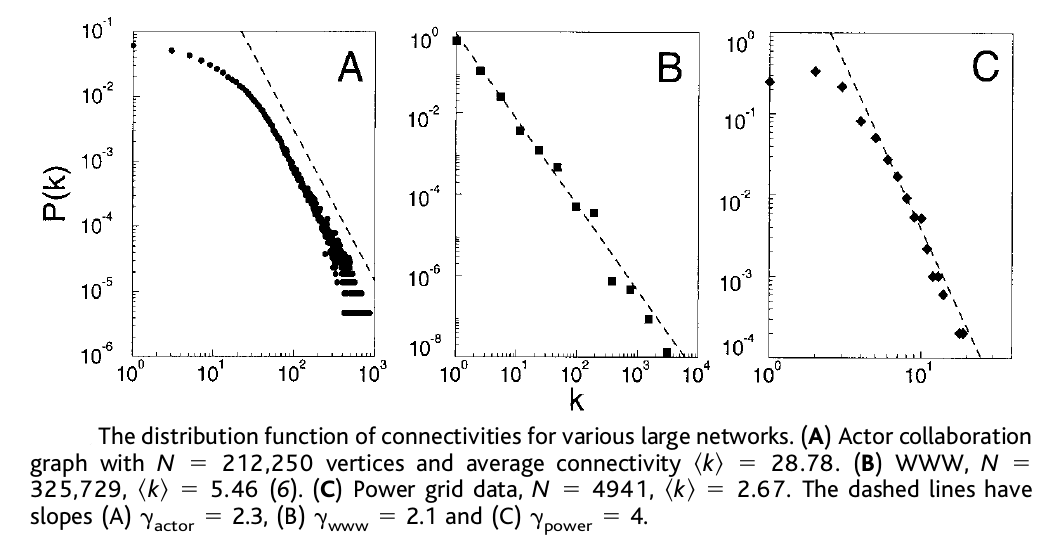
\includegraphics[scale=0.4]{../Images/BAResults.png}
\label{fig:BAGraph}
\caption{The graphs from Barabasi and Albert's 1999 paper show the scale-free structure of a few undirected graphs. $k$ is the average connectivity, or degree, of the vertices in the graph, and $P(k)$ is the proportion of vertices in the graph that have this degree. Plotted on a log-log scale, scale-free networks tend to show long-tailed distributions. This is because a few vertices have the highest degree in the graph.}
\end{figure}

Comparing Figure \ref{fig:BAGraph} to Figure \ref{fig:PunchlineGraph}, we can see that the general structure of both is very similar. This means that the distinct subgraphs we examined are characteristically scale-free. In addition, it means that Wikipedia graphs are well-modeled by the Barabasi-Albert small world graph model.

\begin{figure}[here]
 \centering
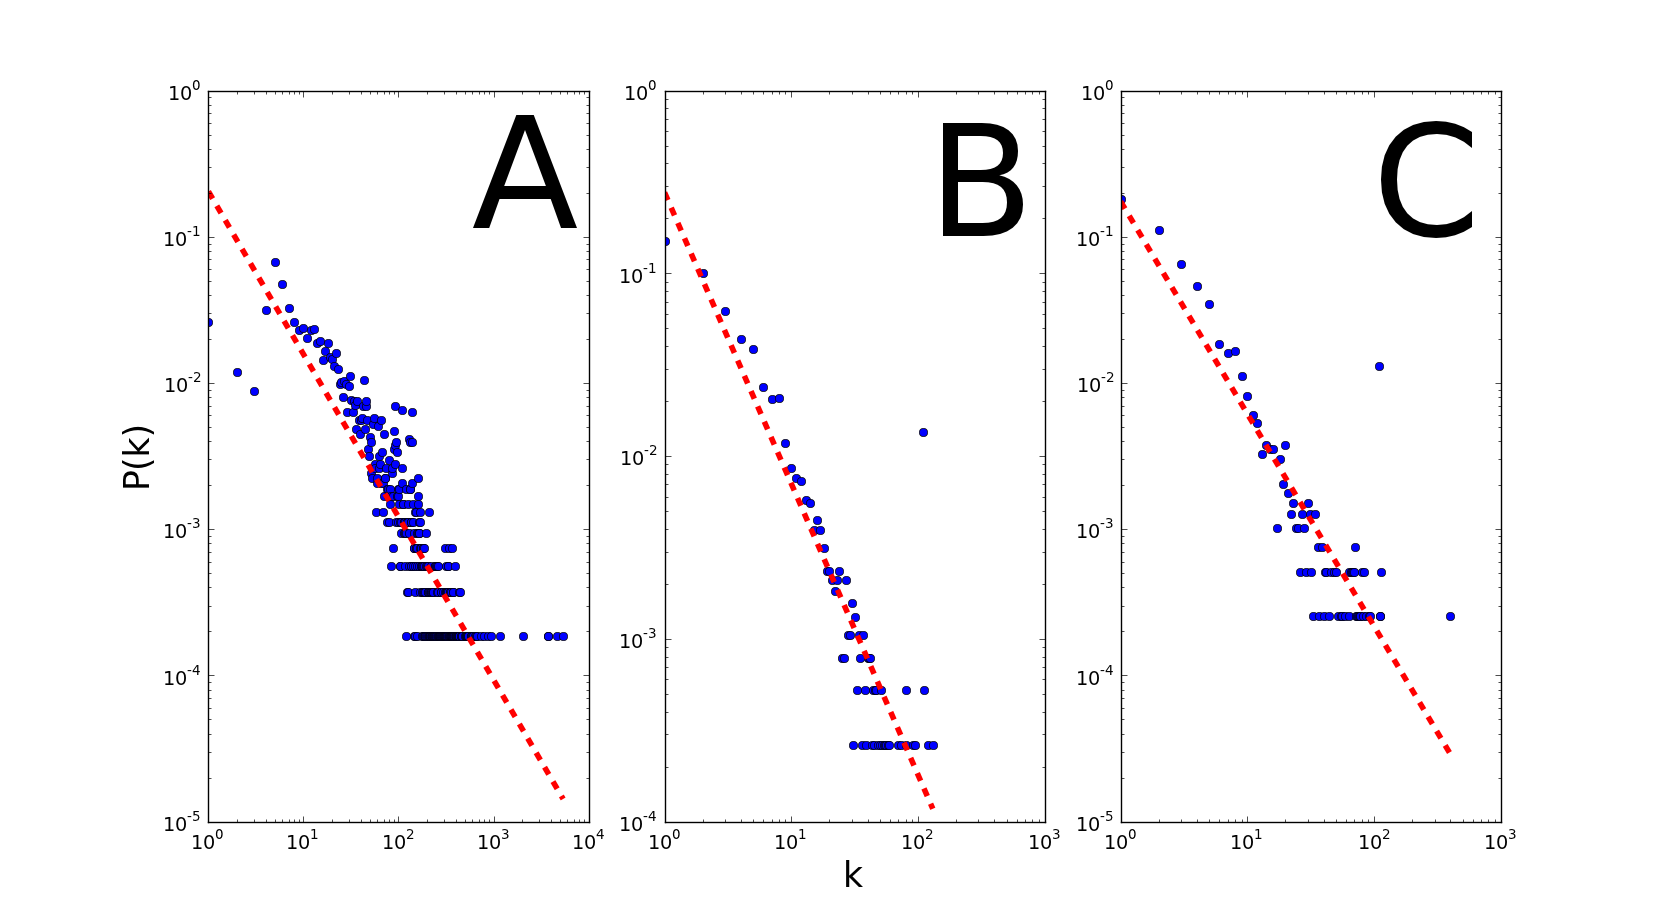
\includegraphics[scale=0.37]{../Images/WikipediaPowerLawGraph.png}
\label{fig:PunchlineGraph}
\caption{The distribution function of connectivities for various large subgraphs of Wikipedia. \textbf{(A)} Index of India-related articles with $N = 5,342$ vertices and average connectivity $ k = 53.56$.  \textbf{(B)} Index of Mathematics articles starting with C, with $N = 3813$ and average connectivity $k = 4.95$. \textbf{(C)} Index of Mathematics articles starting with S, with $N = 3950$ and average connectivity $k = 4.85$. Compared to Figure \ref{fig:BAGraph}, these three graphs also display scale-free distributions. The structure of these distinct subgraphs hints at the nature of Wikipedia as a whole, indicating that Wikipedia is possibly scale-free.}
\end{figure}

But what does this really mean? The Barabasi-Albert model of small world graphs is especially good at modeling preferential attachment, the phenomenon where a few of the vertices have the highest degree. The fact that both the undirected graph of citations in science articles and the directed graph representing Wikipedia have a scale-free distribution of degrees means that preferential attachment is indepedent of the directedness of the graph.

This fact is further explained in Figure \ref{fig:AllThree}, which shows the degree distribution of the in, out, and total degrees of the Index of India-related articles subgraph. All three distributions are scale-free, which means that few vertices have a high in-degree and few vertices have a high out-degree. This corresponds with our findings that preferential attachment is indepedent of the directedness of a graph.

\begin{figure}[here]
 \centering
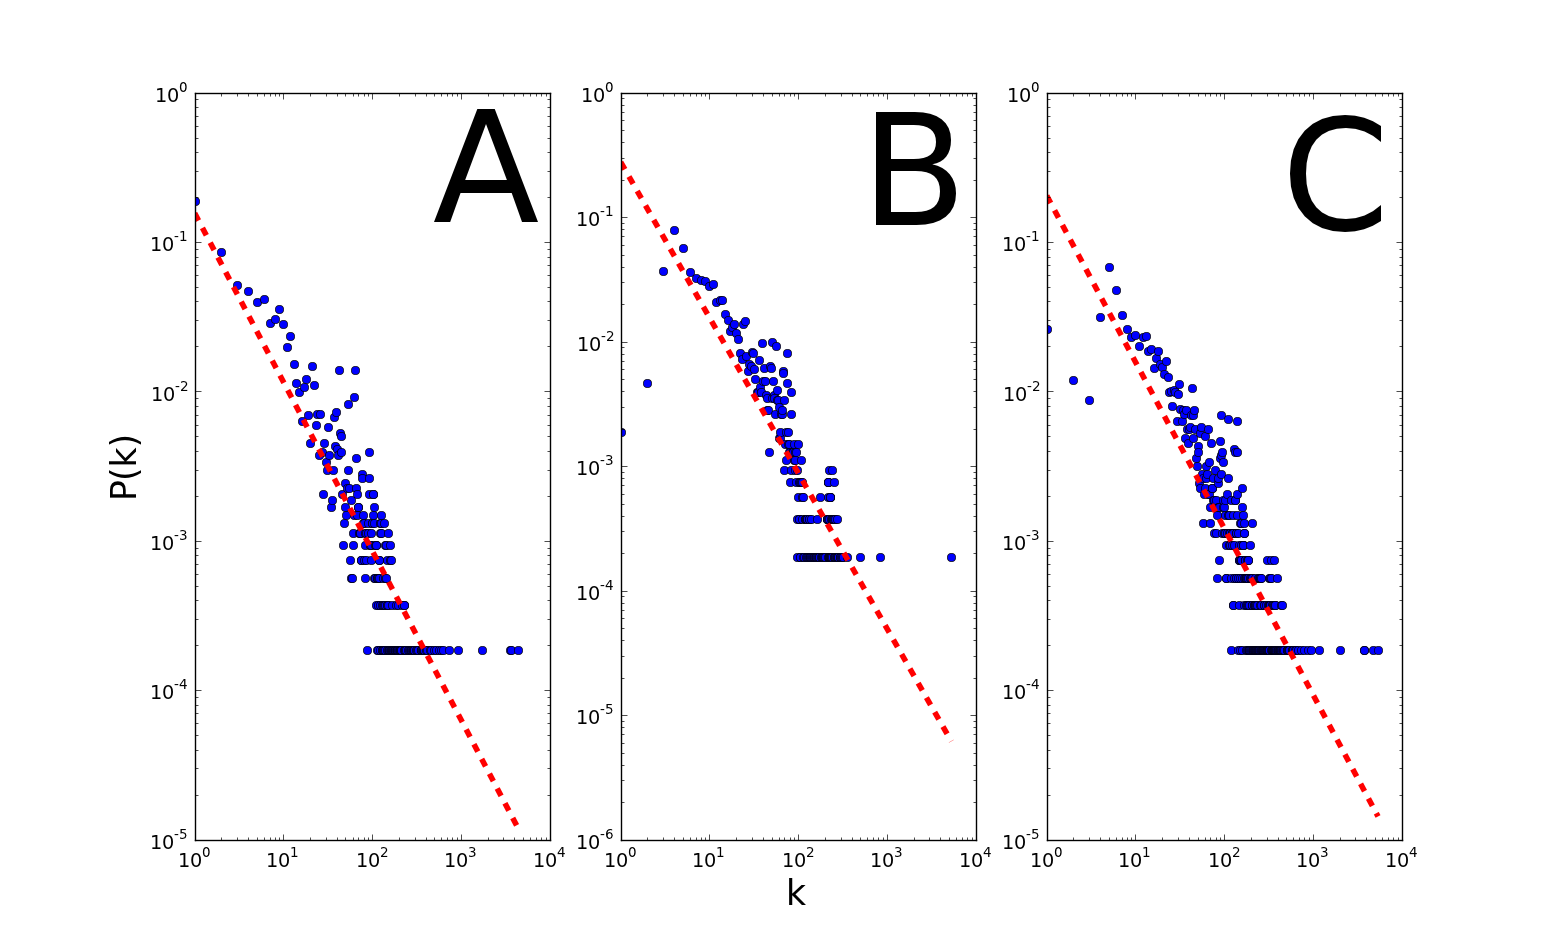
\includegraphics[scale=0.37]{../Images/AllThreeScaleFree.png}
\label{fig:AllThree}
\caption{The distribution function of connectivities for the in-degrees \textbf{(A)}, out-degrees \textbf{(B)}, and total degrees \textbf{(C)} of the vertices in the Index of India-related articles subgraph. Both the in- and out-degree distributions are scale-free, further indicating that preferential attachment is indepedent of directedness.}
\end{figure}

\section{Conclusion}

Since Wikipedia subgraphs display results of preferential attachment, we have another explanation for why you keep landing on the same articles. It could be because there exists a knot in the set of articles you are perusing, but it could also be because that set of articles is very well connected to the rest of the graph. Since subgraphs of Wikipedia are small-world, a small set of vertices will have the highest degrees in the graph. That means that if you take a random walk through the graph, the odds you'll encounter these vertices are very high. 

Barabasi and Albert's example that the undirected graph of citations in science articles indicates that, even if you are traversing an undirected graph, you may encounter the same vertices over and over, without there being a knot. This small set of articles may be cited the most, so in your research for a certain topic, you're very likely to see these articles multiple times.

What does this mean for your research project? Whether you're browsing Wikipedia or JSTOR, you'll end up seeing the same highly-referenced nodes multiple times. In many ways, this can be frustrating when looking for a specific or isolated article, but is a result of the small world nature of the graphs that represent the information you're seeking. 


%---------------Start garbage----------------------%
% Now that we know the odds of finding a knot in Wikipedia, we want to know if this probability is characteristic of solely Wikipedia, or if it’s a property of the types of graphs that Wikipedia resembles. So we tested what kind of graph Wikipedia was. We checked against four types of graphs:
% 1. Truly random graphs, created by the Erdos-Renyi algorithm
% 2. Semi-small world, highly connected graphs, generated by the Watts-Strogatz algorithm
% 3. Truly small world graphs, generated by the Barabasi-Albert algorithm
% 4. None of the above
% 
% Our hypothesis was that the subgraphs we analyzed were characteristically small world graphs. So we plotted the clustering coefficient of the graphs against the number of vertices. The result are in the figure below.
% 
% <insert clustering/vertex figure here />
% 
% The figure indicates that Wikipedia subgraphs cluster in a similar manner to truly small-world graphs. As a result, we generated a sample of Barabasi-Albert graphs similar in size to the 600 Wikipedia graphs we had, and checked the probability that these graphs had a knot. 
% 
% If the probability is similar, discuss implications
% If the probability is not similar, discuss differences between BA and wikipedia




\end{document}